
\documentclass[a4paper,12pt]{article}

\usepackage{a4wide}
%\usepackage[bottom=1cm]{geometry}
%\usepackage{fullpage}
\setlength{\textheight}{23.0cm}
\usepackage{amsmath,amssymb,amsfonts,latexsym,cancel,chemarrow} %Soporte para símbolos y font matemáticos
\usepackage[utf8]{inputenc} % Caracteres con acentos.
\usepackage[spanish,activeacute,es-noshorthands]{babel} % Caracteres con acentos.
\usepackage[bf]{caption} %Caption negrita y chiquita.
\usepackage[T1]{fontenc}
%\usepackage{fouriernc}
\usepackage[sc]{mathpazo}
%\usepackage{anysize} % Soporte para el comando \marginsize
%\marginsize{2cm}{2cm}{2cm}{2cm} %{left}{right}{top}{bottom}
\usepackage{tikz}
\usepackage{gnuplot-lua-tikz}
\usepackage{grffile} %Para leer archivo .algo.pdf
%\usepackage{graphicx}
\usepackage{chemfig}
%\usepackage[lflt]{floatflt}
\usepackage{wrapfig}
\usepackage{setspace}
\onehalfspacing
%\usepackage{fancyhdr}
%\pagestyle{fancy}
\usepackage{array}
\usepackage{multirow}
\usepackage[version=3]{mhchem}
\usepackage{booktabs}
\usepackage{dotlessi}
\usepackage{hyperref}
\usepackage[square, comma, numbers, sort&compress]{natbib}
\usepackage{threeparttable} %Footnotes en las tablas
\usepackage{sidecap} %Side Caption
\usetikzlibrary{calc,3d}
\usepackage{tcolorbox}
\tcbset{colback=blue!25,colframe=blue!75!black,fontupper=\bfseries}

%\fancyhead[LO,RE]{}
%\fancyhead[RO,RE]{Mecánica Estadísitica y Teoría del Estado de Transición}
%\fancyfoot[CO,CE] {\thepage}


\definesubmol\nobond{-[,0.2,,,draw=none]}
\definesubmol{n}{!\nobond\scriptstyle}
\newcommand\scriptchemfig[3][15pt]{\chemmove{\path(#2) node[yshift=-#1]{#3};}}

\newcommand\reaction[1]{\begin{equation}\ce{#1}\end{equation}} %Comando reaction reacción numerada
\newcommand\reactionnonumber[1]% Comando reactionnonumber para reacción nonumerada
  {\begin{equation*}\ce{#1}\end{equation*}}

\usepackage{subfig}
%\setlength{\abovecaptionskip}{-0.5cm}

\interfootnotelinepenalty=10000 %Notas al pie en la misma página

\begin{document}
\title{Teoría del Estado de Transición}
\author{Castillo, M. Ezequiel}
\date{}

\paragraph{Métodos de dinámica acelerada.} 
Incluyen \textit{hiperdinámica, dinámicas de réplicas paralelas y dinámicas
aceleradas por temperatura}. La trayectoria del sistema, atrapada en su estado
actual, es simulada para encontrar una ruta apropiada para escapar más
rápidamente que si lo hiciera con una DM directa. No se necesita información a
priori acerca de cómo es la ruta de escape en el procedimiento; la trajectoria
simplemente sigue su propio camino fuera de su estado.

\paragraph{Sistemas de eventos infrecuentes.}
La evolución dinámica de estos sistemas consiste en excursiones vibracionales
dentro de un valle de potencial, interrumpidas por transiciones ocasionales
entre los valles; estos eventos son infrecuentes en el sentido de que se
necesita en promedio un tiempo muy largo de períodos vibracionales. En algún
punto del tiempo, cuando se localiza la suficiente energía, la trayectoria pasa
a través de una superficie divisoria.

\begin{SCfigure}
	\centering
	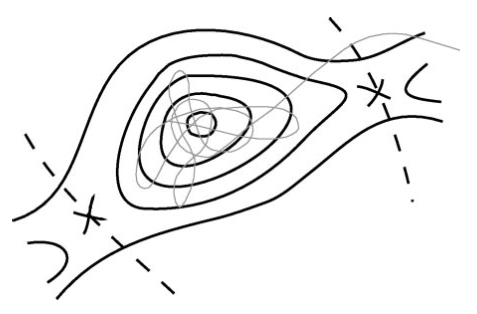
\includegraphics[width=8cm]{fig/basin.png}
	\caption{En esencia, el sistema ``accidentalmente'' escapa del estado y
	una nueva sesión de búsqueda vibracional empieza, sin memoria de cómo
	llegó a ese estado.}
	\label{fig:basin}
\end{SCfigure}


\end{document}
